\documentclass[9pt]{article}
\usepackage[margin=.55in]{geometry}
\usepackage{amsmath,amssymb,xcolor,tikz,fancyvrb,fontspec,multicol}
\usetikzlibrary{arrows.meta,positioning,fit,calc}
\pagestyle{empty}
\setlength{\parindent}{0pt}
\setlength{\parskip}{3pt}
\definecolor{keep}{RGB}{30,105,60}
\definecolor{change}{RGB}{155,55,35}
\definecolor{ink}{RGB}{35,45,70}
\newfontfamily\leanfont{DejaVu Sans Mono}
\newenvironment{lean}{\Verbatim[fontsize=\scriptsize,frame=single,framesep=1.2mm,formatcom=\leanfont]}{\endVerbatim}
\newcommand{\good}{\textcolor{keep}{\bfseries KEEP}}
\newcommand{\edit}{\textcolor{change}{\bfseries TINY EDIT}}
\begin{document}
\begin{center}
 {\Large\bfseries Upstream audit: orbit sums and Frobenius periods}\\[-1mm]
 {\small Lean 4 API shape, proof architecture, and PR split}
\end{center}

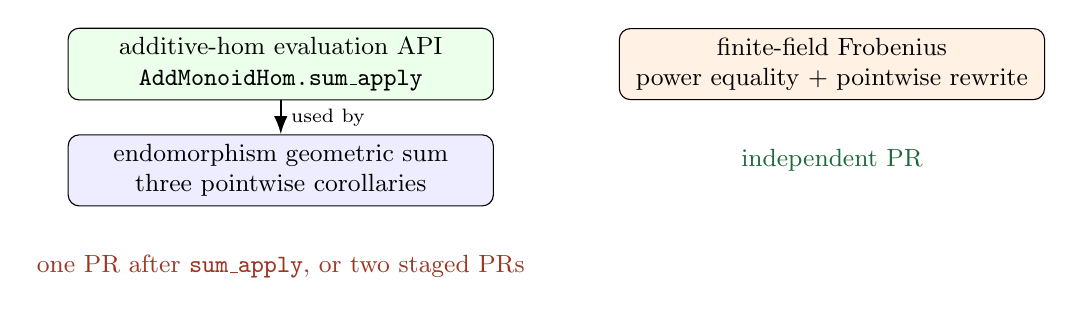
\begin{tikzpicture}[x=1cm,y=1cm,>=Latex,every node/.style={font=\small,align=center}]
\node[draw,rounded corners,fill=green!8,minimum width=5.4cm,minimum height=.8cm] (e) at (3,0)
  {additive-hom evaluation API\\\texttt{AddMonoidHom.sum\_apply}};
\node[draw,rounded corners,fill=blue!7,minimum width=5.4cm,minimum height=.8cm] (g) at (3,-1.35)
  {endomorphism geometric sum\\three pointwise corollaries};
\node[draw,rounded corners,fill=orange!10,minimum width=5.4cm,minimum height=.8cm] (f) at (10,0)
  {finite-field Frobenius\\power equality + pointwise rewrite};
\draw[->,thick] (e)--node[right]{\scriptsize used by}(g);
\node[below=5mm of f,text=keep] {independent PR};
\node[below=5mm of g,text=change] {one PR after \texttt{sum\_apply}, or two staged PRs};
\end{tikzpicture}

\section*{Verdict}
\good\ The mathematical statements and proofs are correct and appropriately generic.  The revised
endomorphism proof now exposes the canonical ring identity instead of re-proving it.  The Frobenius
pair is upstream-ready as written.  Before submission, weaken one unnecessary typeclass assumption
and choose placement that does not burden the foundational endomorphism module with geometric sums.
No global \texttt{[simp]} attribute is recommended.

\begin{multicols}{2}
\section*{1. Generic evaluation lemma}
The abstraction is useful independently of geometric sums:
\begin{lean}
theorem AddMonoidHom.sum_apply
    (f : iota -> A ->+ B) (s : Finset iota) (x : A) :
    (sum i in s, f i) x = sum i in s, f i x
\end{lean}
\edit\ The domain needs only \texttt{[AddMonoid A]}, not
\texttt{[AddCommMonoid A]}.  Commutativity is needed only in the codomain so
that \texttt{A ->+ B} and \texttt{B} support finite sums.

The explicit evaluation hom is preferable to induction and documents why
\texttt{map\_sum} applies:
\begin{lean}
let ev : (A ->+ B) ->+ B :=
  { toFun := fun g => g x
    map_zero' := rfl
    map_add' := fun _ _ => rfl }
exact map_sum ev f s
\end{lean}
\good\ Name, namespace, argument order, and analogy with
\texttt{LinearMap.sum\_apply}.  Put this with additive-hom big-operator API,
not in a finite-field or application file.

\section*{2. Endomorphism geometry}
Let $S_n(x)=\sum_{i=0}^{n-1}\varphi^i(x)$.  Mathlib already knows
\[
 (\varphi-1)\Bigl(\sum_{i<n}\varphi^i\Bigr)=\varphi^n-1
 \quad\text{in }\operatorname{End}(A).
\]
Evaluation gives exactly the requested telescoping law.

\columnbreak
\begin{center}
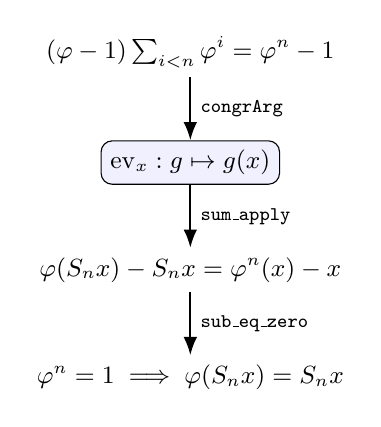
\begin{tikzpicture}[>=Latex,node distance=8mm,every node/.style={font=\small,align=center}]
\node (r) {$ (\varphi-1)\sum_{i<n}\varphi^i=\varphi^n-1$};
\node[below=of r,draw,rounded corners,fill=blue!6] (ev) {$\operatorname{ev}_x:g\mapsto g(x)$};
\node[below=of ev] (p) {$\varphi(S_nx)-S_nx=\varphi^n(x)-x$};
\node[below=of p] (z) {$\varphi^n=1\implies\varphi(S_nx)=S_nx$};
\draw[->,thick] (r)--node[right]{\scriptsize \texttt{congrArg}}(ev);
\draw[->,thick] (ev)--node[right]{\scriptsize \texttt{sum\_apply}}(p);
\draw[->,thick] (p)--node[right]{\scriptsize \texttt{sub\_eq\_zero}}(z);
\end{tikzpicture}
\end{center}

\good\ Keep \texttt{apply\_mul\_geom\_sum} as the coercion bridge; make
\texttt{apply\_sum\_pow\_sub} a thin \texttt{simpa}; derive the fixed-point
lemma by rewriting.  This is canonical and maintainable:
\begin{lean}
have h := congrArg (fun g : AddMonoid.End A => g x)
  (mul_geom_sum phi n)
change (phi - 1) ((sum i in range n, phi ^ i) x) =
  (phi ^ n - 1) x at h
rw [AddMonoidHom.sum_apply
  (fun i => phi ^ i) (range n) x] at h
exact h
\end{lean}

\edit\ Keep these results in a geometric-sum companion module.  Importing
\texttt{Ring.GeomSum} from foundational \texttt{Hom.End} would reverse the
clean dependency direction.  If there is only one downstream consumer, the
first bridge lemma is optional: the displayed \texttt{congrArg} proof is
already short.
\end{multicols}

\newpage
\section*{3. Frobenius periodicity}
For $F=\operatorname{Frob}_p$ and $|K|=p^n$, the existing theorem gives
$F^n=1$.  Generic cyclic reduction then gives $F^m=F^{m\bmod n}$.

\begin{center}
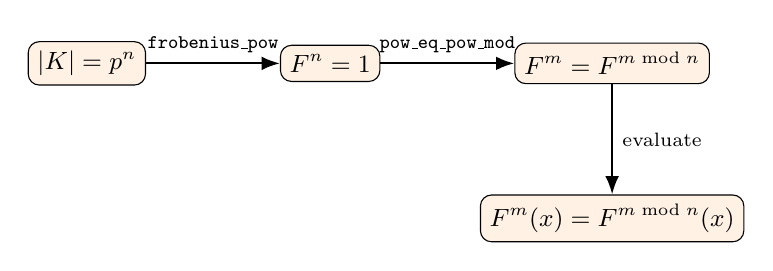
\begin{tikzpicture}[>=Latex,node distance=14mm and 17mm,every node/.style={font=\small,align=center}]
\node[draw,rounded corners,fill=orange!10] (card) {$|K|=p^n$};
\node[draw,rounded corners,fill=orange!10,right=of card] (period) {$F^n=1$};
\node[draw,rounded corners,fill=orange!10,right=of period] (mod) {$F^m=F^{m\bmod n}$};
\node[draw,rounded corners,fill=orange!10,below=of mod] (point) {$F^m(x)=F^{m\bmod n}(x)$};
\draw[->,thick] (card)--node[above]{\scriptsize\texttt{frobenius\_pow}}(period);
\draw[->,thick] (period)--node[above]{\scriptsize\texttt{pow\_eq\_pow\_mod}}(mod);
\draw[->,thick] (mod)--node[right]{\scriptsize evaluate}(point);
\end{tikzpicture}
\end{center}

\begin{multicols}{2}
\good\ The endomorphism equality is the right algebraic API:
\begin{lean}
theorem frobenius_pow_eq_pow_mod
    (hcard : Fintype.card K = p ^ n) (m : Nat) :
    frobenius K p ^ m = frobenius K p ^ (m % n) :=
  pow_eq_pow_mod m (FiniteField.frobenius_pow hcard)
\end{lean}
The pointwise theorem is not redundant: it avoids exposing powers of ring homs
to element-level clients.  Its two rewrites are minimal.

\good\ No hypothesis \texttt{0 < n} is necessary.  At $n=0$,
\texttt{m \% 0 = m}, so the reduction theorem is tautological; for a field,
the cardinality premise $|K|=p^0=1$ cannot occur anyway.

\columnbreak
\good\ The single import \texttt{FieldTheory.Finite.Basic} is enough.
Placement immediately after \texttt{frobenius\_pow} is ideal.
The names distinguish the hom equality from the pointwise rewrite and follow
the surrounding API.

\section*{Merge checklist}
$\square$ weaken \texttt{A} to \texttt{[AddMonoid A]};\\
$\square$ keep geometric sums out of \texttt{Hom.End};\\
$\square$ submit Frobenius independently;\\
$\square$ run formatter, linter, minimum-import check;\\
$\square$ test rewriting in both forms.

\section*{Checked artifact}
The companion Lean target contains all five declarations in the recommended
shape.  It compiles without \texttt{sorry}; theorem-axiom inspection reports
only standard Mathlib axioms.
\end{multicols}

\newpage
\begin{center}
 {\Large\bfseries Additional audit: forward-closed object properties}\\[-1mm]
 {\small Verdict: mathematically sound, but not upstreamable as a parallel interface}
\end{center}

\section*{Blocking duplication}
Mathlib already has the more general class
\begin{lean}
class ObjectProperty.InheritedFromSource
    (P : ObjectProperty C) (Q : MorphismProperty C) : Prop where
  of_hom_of_source {X Y} (f : X -> Y) (hf : Q f) : P X -> P Y
\end{lean}
The submitted notion is precisely the specialization
\[
 \texttt{IsForwardClosed P}
 \quad\simeq\quad
 \texttt{P.InheritedFromSource (top : MorphismProperty C)}.
\]
Therefore a new structure would create two names, two instance ecosystems, and conversion obligations
for the same concept.  This is a blocker for the PR in its present form, not merely a naming preference.

\begin{center}
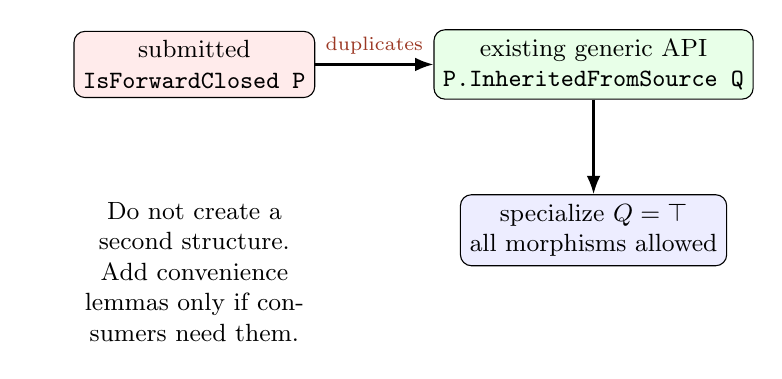
\begin{tikzpicture}[>=Latex,node distance=12mm and 15mm,every node/.style={font=\small,align=center}]
\node[draw,rounded corners,fill=red!8] (new) {submitted\\\texttt{IsForwardClosed P}};
\node[draw,rounded corners,fill=green!9,right=of new] (old)
  {existing generic API\\\texttt{P.InheritedFromSource Q}};
\node[draw,rounded corners,fill=blue!7,below=of old] (spec)
  {specialize $Q=\top$\\all morphisms allowed};
\draw[->,thick,text=change] (new)--node[above]{\scriptsize duplicates}(old);
\draw[->,thick] (old)--(spec);
\node[below=of new,text width=4cm] {Do not create a second structure.\\Add convenience lemmas only if consumers need them.};
\end{tikzpicture}
\end{center}

\begin{multicols}{2}
\section*{How each declaration maps}
\begin{itemize}\setlength\itemsep{2pt}
\item \texttt{map}: use \texttt{P.of\_hom\_of\_source f trivial} with
  $Q=\top$; a short wrapper such as \texttt{prop\_of\_hom} may be worthwhile.
\item \texttt{iso\_iff}: derive isomorphism closure from the existing class;
  then use \texttt{P.prop\_iff\_of\_iso e}.  A direct two-arrow proof is fine.
\item \texttt{and}: already an instance for $(P\sqcap Q)$; use lattice notation
  rather than \texttt{fun X => P X \& Q X}.
\item \texttt{top}: add a generic top-object-property instance in the existing
  namespace if actual reuse warrants it.
\item \texttt{inverseImage}: the useful missing theorem is more general:
  pull back both the object property and $Q$ along a functor.
\item natural transformation and terminal results are tiny corollaries of the
  all-morphisms specialization; keep downstream unless repeated consumers appear.
\end{itemize}

\columnbreak
\section*{Recommended generic addition}
Instead of the proposed file, consider one instance in
\texttt{ObjectProperty/InheritedFromHom.lean}:
\begin{lean}
instance inverseImage (F : D => C)
    [P.InheritedFromSource Q] :
    (P.inverseImage F).InheritedFromSource
      (Q.inverseImage F) where
  of_hom_of_source f hf :=
    P.of_hom_of_source (F.map f) hf
\end{lean}
Here the displayed arrows abbreviate Lean's functor notation.  This statement
subsumes the submitted inverse-image result and remains useful for monomorphisms,
epimorphisms, weak equivalences, and other restricted classes.

\section*{API/style notes}
If a top-specialized convenience layer is accepted, follow existing style:
make closure a \texttt{class}, make canonical constructions \texttt{instance}s,
and use implicit typeclass arguments rather than passing \texttt{hP} explicitly.
Import \texttt{ObjectProperty.InheritedFromHom}, not merely \texttt{Basic}.
The name ``inherited from source'' is already established and avoids ambiguity
about ``forward.''

\section*{Strength of the notion}
With an initial object, $P(\bot)$ forces $P$ on every object.  Thus inheritance
along all arrows is strong; examples should establish recurring use.

\section*{Final recommendation}
\textbf{Do not upstream the submitted structure/file.}  Rebase on
\texttt{InheritedFromSource}.  A small PR adding the generic inverse-image
instance and perhaps one top-specialized transport lemma could be upstreamable;
leave the natural-transformation and terminal one-liners downstream until reused.
The submitted code itself was build-checked and contains no proof gap.
\end{multicols}
\end{document}
